\section{Arsitektur Sistem Operasi Linux}
\subsection{Kernel}
	Kernel Linux merupakan kernel yang digunakan dalam sistem operasi GNU/Linux. Kernel ini merupakan turunan dari sistem operasi UNIX, yang mana di rilis menggunakan lisensi GNU \textit{General Public License} (GPL) dan dikembangkan oleh programmer di selururh dunia karena sifatnya yang \textit{open source}. Kernel ini merupakan inti dari sistem operasi komputer dengan memiliki kontrol penuh atas segala dalam sistem tersebut. Kernel ini menghubungkan antara perangkat lunak dan perangkat keras seperti pada gambar \textbf{\ref{kernel}}, salah satu program pertama yang memuat fungsi kernel ini yaitu dimuat didalam start-up setelah proses bootloader.

\begin{figure}[!htbp]
\centerline{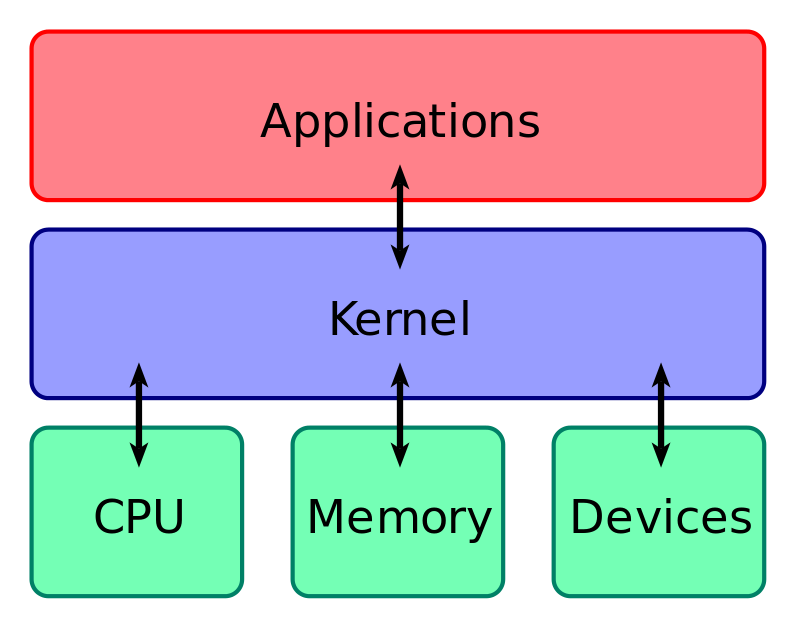
\includegraphics[width=0.75\textwidth]{Figures/Kernel_Layout.png}}
\caption{Kernel connect}
\label{kernel}
\end{figure}

\lstinputlisting[caption=contoh dasar kode program kerne membuat hello world,label={lst:kode dasar}]{src/contoh.tex}

\subsection{struktur data kernel}
	Ketika kernel melakukan sebuah proses, data-data proses tersebut akan disimpan secara periodik ke dalam bentuk file-file. Untuk dapat melihat data kernel, maka file-file tersebut harus diparsing setiap saat dikarenakan datanya yang dinamis \cite{raharja2001pengenalan}. Cara termudah untuk melakukan hal tersebut yaitu menggunakan perintah \textbf{cat} \ref{lst:kode dasar2}

\lstinputlisting[caption=Perintah cat pada linux,label={lst:kode dasar2}]{src/cat.sh}
File-file ini akan tersimpan di dalam direktori yang tersetruktur dalam direktori /proc.

\subsection{Instalasi}
Setelah kita memahami tentang kernel dan juga struktur data kernel, selanjutnya kita akan mencoba install kernel sebelum itu kita dapat cek versi kernel kita dengan mengetikan pada terminal 
\begin{verbatim}
$ uname -r 
\end{verbatim}
\textbf{uname} ini merupakan perintah untuk mengetahui sistem informasi dan \textbf{-r} merupakan perintah untuk menampilkan versi kernel.
 
Untuk instalasi sendiri terdapat beberapa cara yaitu kamu bisa mendownload package dan mencompile dari sumber atau bisa juga hasil download package management tools.
dengan mengetikan pada terminal
\begin{verbatim}
$ sudo apt install linux-generic-lts-vivid
\end{verbatim}
 sebagai contoh : \textbf{sudo apt install 3.19.0-43-generic} setelah itu tinggal reboot maka kernel yang kita compile tadi akan terinstall.
cara alternatif selain itu kita dapat langsung meng-\textit{upgrade} versi kernel dengan menggunakan \textbf{dist-upgrade} maka itu akan mengupdate semua package di dalam sistem. 
 \begin{verbatim}
$ sudo apt dist-upgrade
\end{verbatim}

Setelah melakukan penginstalan sebuah kernel, maka itu akan menambah beberapa file system yang ditambahkan di direktori /boot
kamu akan mendapatkan beberapa file untuk versi kernel yang berbeda seperti :
\begin{enumerate}
\item \textbf{vmlinuz} - ini adalah kernel linux yang sebenarnya
\item \textbf{initrd} - ini digunakan sebagai sistem berkas sementara sebelum memuat kernel
\item \textbf{system.map} - ini sebagai table simbol 
\item \textbf{config} - ini sebagai pengaturan kernel, jika kamu mencompile kernel sendiri maka kamu dapat mengatur modul-modul yang dimuat
\end{enumerate}
Ketika direktori /boot kehabisan ruang penyimpanan, kamu dapat menghapus versi lama dari file-file atau package yang lama. Tapi harus berhati-hati ketika melakukan pemeliharaan di dalam direktori ini karena ditakutkan akan menghapus kernel yang digunakan secara tidak sengaja.

\subsection{Shell}
\subsubsection{Pengertian}
Shell menyediakan sebuah antarmuka untuk sistem unix, untuk mengumpulkan masukan yang diinputkan dan menjalankan program berdasarkan apa yang kita input. Ketika program dieksekusi , maka akan menampilkan \textit{output} sebuah program. 
jadi, shell ini dapat kita artikan sebagai sebuah lingkungan dimana kita dapat menjalankan perintah, program, dan \textit{shell scripts}.
shell menetapkan sendiri perintah dan fungsi sebagai berikut :
\begin{enumerate}
\item \textbf{Shell Prompt}
prompt,\$, atau yang biasa kita sebut \textit{command prompt}, Shell ini membaca \textit{inputan} kalian setelah anda tekan \textbf{Enter}, lalu perintah tersebut akan dieksekusi dengan melihat kata pertama dari inputan kalian.
Contoh sederhana dari \textit{\textbf{date} command}, yang mana akan menampilkan tanggal dan waktu sebagai berikut :
\begin{verbatim}
$date
\end{verbatim}

\item{Shell Types}
terdapat 2 tipe shells yaitu :
\begin{itemize}
\item Bourne shell, Jika kalian menggunakan Bourne-type shell, karakter \$ merupakan default prompt 
Bourne shell memiliki sub kategori sebagai berikut :
\subitem Bourne shell (sh)
\subitem Korn shell (ksh)
\subitem Bourne Again Shell (bash)
\subitem Posix shell (sh)
\item C shell, jika kalian menggunakan C-type shell, karakter \% merupakan default prompt
 sedangkan C shell memiliki sub kategori 
\subitem c shell (csh)
\subitem Tenex/TOPS C shell (tcsh)
\end{itemize}

\item{shell script}
konsep dasar dari shell script selalu diawali dengan tanda \# yang menggambarkan langkah-langkah
Contoh script 
kita asumsikan membuat sebuah test.sh seperti berikut :
\begin{verbatim}
#!/bin/sh
\end{verbatim}
perintah tersebut biasa disebut shebang, yang mana simbol \# disebut hash dan ! disebut bang.
Untuk membuat script yang terdapat perintah ini, kalian harus menetapkan \textit{shebang} di baris pertama dan selanjutnya diikuti dengan perintah tambahan seperti berikut
\begin{verbatim}
#!/bin/bash
pwd
ls
\end{verbatim}
\end{enumerate}

\subsection{Commands and Utilities}
Terdapat berbagai perintah dan utilitas yang kalian dapat gunakan, ada lebih dari 250 perintah standar plus dengan yang disediakan melalui \textit{software} dari pihak ke-3. 

Beberapa perintah yang biasa digunakan sebagai berikut :

\begin{table}[h]
		\caption{Perintah dasar Unix}
		\label{commands}
			\begin{tabular}{|c|l|}
			\hline
			\textbf{Perintah}& \textbf{Keterangan} \\
			\hline
			cat&Perintah yang digunakan untuk membaca, memodifikasi atau concatenate file teks\\
			\hline
			cd&Perintah untuk mengubah direktori saat ini dan berpindah ke direktori yang ditentukan\\
			\hline
			chmod&Perintah untuk mengubah ijin dari satu atau lebih file\\
			\hline
			cp&Perintah untuk mencopy files dan direktori\\
			\hline
			df&Perintah untuk menampilkan jumlah ruang penyimpanan yang tersedia pada sistem file yang mengandung argumen setiap nama file\\
			\hline
			env&Perintah ini untuk menjalankan program environment yang dimodifikasi\\
			\hline
			ifconfig&Perintah ini digunakan untuk mengkonfigurasi antarmuka jaringan kernel,hal ini biasanya hanya digunakan ketika debugging atau sistem tuning\\
			\hline
			ifup&Perintah ini digunakan admin untuk mengkonfigurasi antarmuka jaringan dan mengaktifkan koneksi jaringan\\
			\hline
			ifdown&Perintah ini digunakan untuk menutup antarmuka jaringan dan menonaktifkan koneksi jaringan\\
			\hline
			iptables&Perintah yang memungkinkan atau blok lalu-lintas pada linux host dan dapat mencegah aplikasi tertentu dari menerima atau mengirimkan permintaan\\ 
			\hline
			kill&Perintah ini digunakan mematikan proses atau aplikasi dengan aman\\
			\hline
			ls&Perintah untuk menampilkan daftar file dan direktori\\
			\hline
			mkdir&Perintah ini digunakan untuk membuat direktori baru dengan nama path\\
			\hline
			netconfig/netcfg&Perintah ini digunakan untuk menkonfigurasi jaringan, mengaktifkan produk-produk jaringan dan menampilkan informasi konfigurasi jaringan\\
			\hline
			netstat&Perintah ini digunakan untuk menyediakan informasi dan statistik tentang protokol dalam penggunaan dan koneksi jaringan TCP/IP,untuk mengetahui proses dan program yang aktif pada komputer dan yang terdapat dalam satu jaringan\\
			\hline
			 nslookup&Perintah ini digunakan untuk dapat memasukkan nama dan menemukan IP sesuai dengan nslookup, berguna untuk membantu menemukan nama host\\
			\hline
			passwd&Perintah ini digunakan untuk memperbarui sandi pengguna saat ini\\
			\hline
			ping&Perintah ini digunakan untuk memverifikasi alamat IP tertentu dan dapat menerima permintaan IP, selain itu digunakan untuk menguji konektivitas dan menentukan waktu respon serta memastikan pengguna bahwa host bekerja\\
			\hline
			ps&Perintah ini digunakan untuk melaporkan status proses saat ini dalam sistem\\
			\hline
			pwd&Perintah ini digunakan untuk menampilkan nama direktori yang sedang dijalankan saat ini\\
			\hline
			sudo&Perintah ini digunakan untuk memungkinkan administrasi sistem yang memberikan user kemampuan untuk menjalankan beberapa aatau semua perintah dan argument\\
			\hline
			ssh&Perintah ini digunakan untuk mengakses remote komputer yang aman dan digunakan admin meremote kontrol server\\
			\hline
			uname&Perintah ini digunakan untuk menampilkan nama sistem operasi saat ini dan dapat mencetak inforamsi sistem\\
			\hline
			vi&Perintah ini digunakan sebagai teks editor yang memungkinkan pengguna untuk mengontrol sistem dengan hanya keyboard, mouse dan penekanan tombol \\
			\hline
			vmstat&Perintah ini digunakan untuk menampilkan sistem dan laporan informasi tentang berbagai proses, memori, paging dan aktivitas CPU. selain itu metode ini digunakan untuk menentukan mana masalah perlambatan dapat terjadi dalam sistem\\
			\hline
			wget&Perintah ini digunakan untuk utilitas jaringan dalam mengambil file web yang mendukung HTTP, HTTPS dan protokol FTP\\
			\hline
		\end{tabular}
		\end{table}

\subsection{Struktur direktori Linux}
Pada direktori root linux terdapat beberapa direktori standar yang biasa ada pada banyak distro linux, direktori tersebut sebagai berikut :
\begin{table}[h]
		\caption{Direktori Linux}
		\label{direktori}
			\begin{tabular}{|c|l|}
			\hline
			\textbf{Direktori}& \textbf{Isi} \\
			\hline
			/bin&Berisi file-file binary standar yang dapat digunakan oleh seluruh user \\
			\hline
			/boot&Berisi file-file yang digunakan untuk booting Linux termasuk kernel image\\
			\hline
			/dev& Berisi file system khusus yang merupakan refleksi device hardware yang dikenali dan digunakan sistem \\
			\hline
			/etc&Berisi file-file konfigurasi sistem, biasanya hanya boleh diubah oleh super user\\
			\hline
			/home&Berisi direktori-direktori yang merupakan direktori home untuk user biasa dan aplikasi tertentu\\
			\hline
			/lib&Berisi file-file library yang digunakan untuk mendukung kerja kernel Linux\\
			\hline
			/mnt&Direktori khusus yang disediakan untuk mounting (mengaitkan) device disk storage ke sistem dalam bentuk direktori \\
			\hline
			/prod&Berisi file system khusus yang menunjukkan data-data kernel setiap saat\\
			\hline
			/root&Direktori home untuk user root (user khusus dengan priviledges hampir tak terbatas)\\
			\hline
			/sbin&Sama halnya dengan direktori bin, tetapi hanya super user yang sebaiknya menggunakan binary-binary tersebut mengingat fungsi-fungsi binary yang terdapat di direktori ini untuk maintenance sistem\\
			\hline
			/tmp&Berisi file-file sementara yang dibutuhkan sebuah aplikasi yang sedang berjalan\\
			\hline
			/usr&Berisi library, binary, dokumentasi dan file lainnya hasil instalasi user\\
			\hline
			/var&Berisi file-file log, mailbox dan data-data aplikasi\\
			\hline
		\end{tabular}
		\end{table}